\documentclass[11pt]{amsart}

\usepackage[english]{babel}
\usepackage {amsmath} 
\usepackage{amssymb}
\usepackage{amsfonts}
\usepackage{amsthm}
\usepackage{graphicx}
\usepackage[dvipsnames]{xcolor}
\usepackage{lipsum}
\usepackage[colorlinks,linkcolor=blue, citecolor=blue,urlcolor=blue]{hyperref}
\usepackage[backend=bibtex]{biblatex}
\usepackage[colorinlistoftodos]{todonotes}

\newcommand{\info}[1]{\todo[linecolor=OliveGreen,backgroundcolor=OliveGreen!25,bordercolor=OliveGreen]{#1}}
\newcommand{\unsure}[1]{\todo[linecolor=red,backgroundcolor=red!25,bordercolor=red]{#1}}
\newcommand{\change}[1]{\todo[linecolor=Plum,backgroundcolor=Plum!25,bordercolor=Plum]{#1}}

%% Environments for theorems, etc.. 
\theoremstyle{theorem} % set the style for the following theorems
\newtheorem{thm}{Theorem}[section] %\newtheorem{name}{display-text}[numbered-within]
\newtheorem{lem}[thm]{Lemma} %\newtheorem{name}[numbered-like]{display-text}
\newtheorem{cor}[thm]{Corollary}
\newtheorem{prop}[thm]{Proposition}
\newtheorem{alg}[thm]{Algorithm}
\theoremstyle{definition}       
\newtheorem{defn}[thm]{Definition}
\newtheorem{conj}[thm]{Conjecture}
\theoremstyle{example}                     
\newtheorem{prob}[thm]{Problem}
\theoremstyle{remark}                       
\newtheorem{exmp}[thm]{Example}
\newtheorem{rem}[thm]{Remark}
\newtheorem{claim}[thm]{Claim}  
\renewcommand{\theclaim}{}

\numberwithin{equation}{section}

\newcommand{\R}{\mathbb{R}}
\newcommand{\Q}{\mathbb{Q}}
\newcommand{\N}{\mathbb{N}}
\newcommand{\Z}{\mathbb{Z}}
\DeclareMathOperator{\rank}{rank}
\DeclareMathOperator{\dimension}{dim}
\DeclareMathOperator*{\supp}{supp}

\addbibresource{wavelet.bib}

\title{Introduction to Wavelets in Image Processing}
\author{Jason Ngo}
\date{2019-04-03}

\begin{document}
\maketitle

\section{Introduction}
Since the start of the 20th century, we have seen rapid development in the theory and applications of wavelets. As a mathematical tool, wavelets can be used to extract information from different kinds of data such as audio signals and images.

This paper will explore what wavelets are, introduce readers to the Haar wavelet basis, approximate functions using Haar wavelets, and discuss their applications in image compression.

\section{Definitions}
\info{Cite this section.}
\begin{defn} \label{def:l2}
	\emph{$ L^2(\R) $} is a normed vector space of all functions $ f: \R \to \R $ such that the integral of $ f^2 $ over $ \R $ is finite, taken with the norm
	\[ \|f\|_2 = \left( \int_{\R} |f(x)|^2 dx \right)^{\frac{1}{2}}, \]
	and the inner product
	\[ \langle f,g \rangle = \int_{\R} f(x) g(x)  dx. \]
\end{defn}

\begin{defn} \label{def:orthonormal}
	A set of functions $ \{ \varphi \}_{k=1}^N $ is said to be an \emph{orthonormal basis} for the N-dimensional space $ V $ if:
	\begin{enumerate}
		\item Every $ u \in V $ can be written as $ u = \sum_{k=1}^N c_k \varphi_k $ for some scalar $ c_k $\footnote{We can easily prove that $ c_k = \langle u,\varphi_k \rangle $, for $ k = 1,2,\cdots,N. $}.
		\item $ \langle \varphi_j, \varphi_k \rangle = 0 $ if $ j \neq k $.
		\item $ \langle \varphi_j, \varphi_k \rangle = 1 $ if $ j = k $.
	\end{enumerate}
\end{defn}

\begin{defn} \label{def:support}
	The \emph{support} of a real-valued function $ f $ is the subset of the domain containing those elements which are not mapped to zero.	
	
	For example, the \emph{support} of the Haar wavelet, denoted $ \supp \varPsi $, is $ [0,1] $.
\end{defn}

\begin{defn} \label{def: wavelet}
	A \emph{wavelet} is a function $ \varPsi \in L^2(\R) $ such that the set
	\[ \{ \varPsi_{j,k}(x) = 2^{j/2} \varPsi (2^j x-k): j,k \in \Z  \} \]
	forms an orthonormal basis for $ L^2(\R) $. Sometimes $ \varPsi $ is called the \emph{mother wavelet}.
\end{defn}

This paragraph is from \cite{frazier}. The factor of $ 2^{j/2} $ in the definition is included so that the $ L^2 $ norms will be the same for all $ j,k $:
		\begin{align*}
			\| \varPsi_{j,k} \|^2 = \int_{\R} \left| 2^{j/2} \varPsi(2^{j} x - k) \right|^2 dx 
			&=   \int_{\R} 2^j \left| \varPsi(2^{j} x - k) \right|^2 dx \\
			&= \int_{\R} \left| \varPsi(y) \right|^2 dy
			= \| \varPsi \|^2,
		\end{align*}
		by change of variable $ y = 2^{j}x-k $ in the integral.
	
Now, let us explore one particular type of wavelet that has many applications in noise filtering and image processing: \emph{The Haar Wavelet}.

\begin{defn}
	The \emph{Haar wavelet} is the function $ \varPsi = \chi_{[0,0.5)} - \chi_{[0.5,1)} $, where $ \chi $ is the characteristic function. The \emph{Haar wavelet basis is the family $ \{ \varPsi_{j,k}:j,k \in \Z \} $}.
\end{defn}
See Figure \ref{fig:haarsystem} for examples of some elements of the Haar wavelet basis, obtained by translating and/or stretching the Haar wavelet. 

\begin{figure}
	\centering
	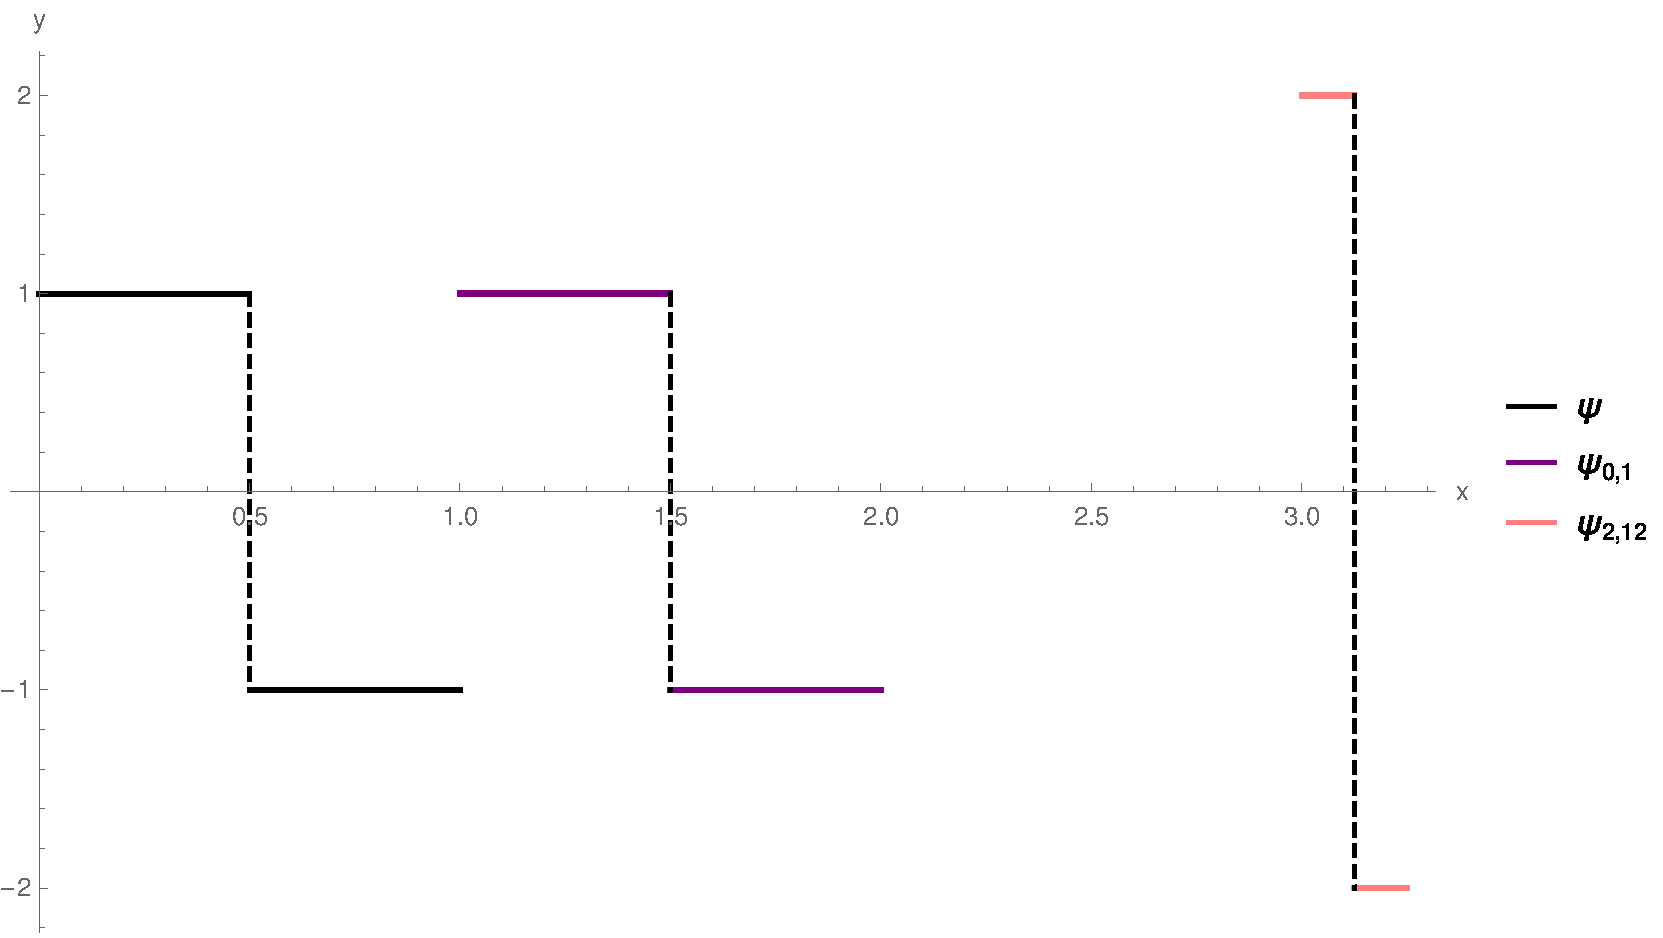
\includegraphics[width=0.7\linewidth]{img/haar_system}
	\caption[Elements of the Haar system]{Elements of the Haar system: $ \varPsi, \varPsi_{0,1} $ and $ \varPsi_{2,12} $}
	\label{fig:haarsystem}
\end{figure}

Note that $ \varPsi_{j,k} $ has width of order $ 2^{-j} $, and is centered about $ k 2^{-j} $. We can see that the Haar wavelet $ \varPsi $ has the following properties:
\begin{enumerate}
	\item $ \int_{\R} \varPsi(x)dx = 0 $, which makes it a wave.
	\item  $ \int_{\R} \varPsi(x)^2dx = 1 $, i.e. the norm is 1.
\end{enumerate}

Now, our task is to prove that the Haar wavelet is in fact a wavelet, i.e. the Haar wavelet basis is an orthonormal basis for $ L^2(\R) $.


\section{Haar wavelet basis}
\begin{lem}
	The Haar system is an orthonormal set in $ L^2(\R) $.
	
	\begin{proof}
		First, we compute the norm of an arbitrary element in the Haar wavelet basis: \info{Consider explaining why $ \| \varPsi (2^j x) = 1 \| $ if it's not obvious.}
		\begin{align*}
			\| \varPsi_{j,k} \|^2_2 &= \int_{\R} \left( 2^{j/2} \varPsi(2^{j} x - k) \right)^2 dx \\
			&= 2^j  \int_{\R} \left( \varPsi(2^{j} x - k) \right)^2 dx \\
			&= 2^j \int_{\R} \left( \varPsi(2^{j} x) \right)^2 dx \\
			&= 2^j \| \varPsi(2^jx) \| =  2^j \frac{1}{2^j} = 1.
		\end{align*}
		Now, we want to show that the Haar system is orthogonal. Consider $ \varPsi_{j,k} $ and $ \varPsi_{j,k'} $, for $ k \neq k' $. Since these two elements have disjoint support, their inner product is 0. \unsure{More explanation needed.} If $ j < j' $, then either $ \varPsi_{j,k} $ and $ \varPsi_{j',k'} $ have disjoint supports, or supp $ \varPsi_{j',k'} $ is contained in an interval on which $ \varPsi_{j,k} $ is constant. In either case $ \langle \rangle = 0 $.
	\end{proof}
\end{lem}

\begin{defn}
	Set $ \varphi = \chi_{[0,1)} $. Define the sequence of partial sums $ H_nf $ to be:
	\[ H_n f(x) = \langle f, \varphi \rangle \varphi(x) + \sum_{j=0}^{n-1} \sum_{k=0}^{2^j-1} \langle f, \varPsi_{j,k} \rangle \varPsi_{j,k} (x). \]
\end{defn}

\begin{lem}
	Let $ f \in L^2(0,1) $. Then $ H_nf $ converges to $ f $ in the $ L^2 $ norm. Consequently, the Haar system is an orthonormal basis for $ L^2(0,1) $. Moreover, if $ f $ is continuous on $ [0,1] $, then $ H_nf $ converges uniformly to $ f $.
\end{lem}

\begin{thm}
	The Haar wavelet basis spans all of $ L^2(\R) $.
\end{thm}

\section{Approximations using Haar wavelets}
\begin{thm}
	If $ f \in C_0(\R) $, then the series $ \sum_{j,k \in \Z} \langle f, \varPsi_{j,k} \rangle \varPsi_{j,k} $ converges to $ f $ uniformly on $ \R $.
\end{thm}

\begin{exmp}
	Consider $ f(x) = e^{-x} \sin 2\pi x $ for $ x \in (0,1) $.
	
	See Figure \ref{fig:approximations} 
\end{exmp}

\begin{figure}
	\centering
	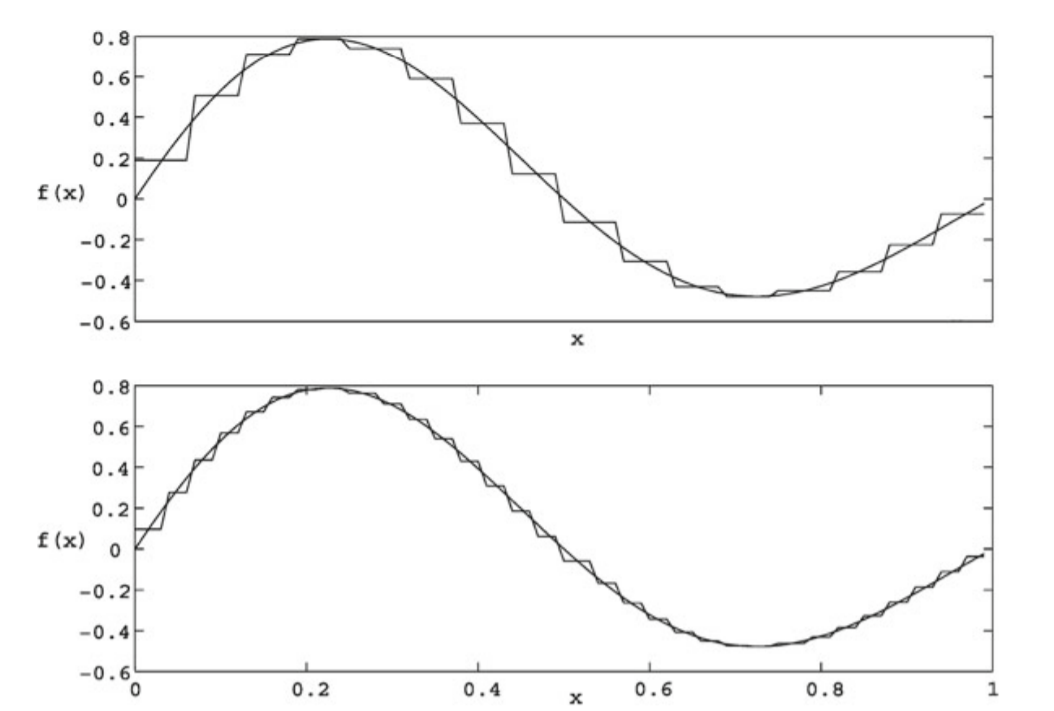
\includegraphics[width=0.7\linewidth]{img/approximations}
	\caption{Approximations of $ f(x) = e^{-x} \sin{2\pi x} $ using Haar wavelets}
	\label{fig:approximations}
\end{figure}


\section{Application to Image Processing}
 When compressing images, we want to discard the least significant details, keeping the original picture largely intact. Fortunately, wavelets can isolate and decompose a signal into low frequency part and high frequency part.
 Briefly discuss FBI Fingerprint Image Compression if there is space:
 \begin{quote}
 	 Wavelet compression methods do not require dividing the image into smaller blocks because the desired localization properties are naturally built into the wavelet system.\cite{frazier}
 \end{quote}



\end{document}

